\chapter{Analisi dei requisiti}
\label{cap:analisi-requisiti}

\intro{In questo capitolo viene esposta l'analisi dei requisiti effettuata durante lo stage, dove si
 vanno ad illustrare le funzionalità tramite casi d'uso e requisiti identificati, con l'obiettivo di creare un'immagine
 più chiara e definita del sistema.
 }\\
 
\section{Descrizione dell'applicazione}

Il progetto consiste nel creare un portale che permetta la consultazione di tutte le API Thron con la possibilità di provarle in modo semplice e veloce, direttamente dal portale.
Il prodotto verrà utilizzato internamente all'azienda, all'interno della Product Area, con lo scopo di facilitare attività di sviluppo, di testing e di supporto durante le attività giornaliere aziendali.

\section{Casi d'uso}\label{sec:usecase}
Questa sezione illustra i casi d'uso individuati nel corso dell'analisi dei requisiti del progetto che sono stati definiti utilizzando il linguaggio Unified Modeling Language (UML).
Ogni caso d'uso offre una panoramica chiara dei diversi attori coinvolti e delle intereazioni che essi intraprendono nel contesto del sistema.\\

Ogni caso d'uso è indentificato da un codice univoco, che segue la seguente notazione:
\begin{center}
    \textbf{UC[Codice-padre].[Codice-figlio]}
  \end{center}

% \clearpage

\subsection{Attori}
Gli attori individuati nel sistema sono i seguenti visibili in figura \ref{fig:attori-individuati}, più in dettaglio:
\begin{itemize}
    \item Utente non autenticato: è un utente che non è autenticato nel sistema e non può accedere alle funzionalità del portale;
    \item Utente autenticato: è un utente che è autenticato nel sistema e che può accedere alle funzionalità del portale.
\end{itemize}

\begin{figure}[h] 
    \centering 
    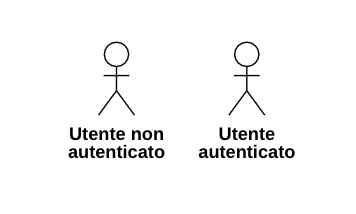
\includegraphics[width=0.5\columnwidth, alt={Attori individuati nel sistema}]{images/usecase/attori.jpg}
    \caption{Attori individuati}\label{fig:attori-individuati}
\end{figure}\\

% \clearpage


\subsection{Descrizione del sistema}

Di seguito viene illustrato un diagramma riassuntivo che mostra i casi d'uso individuati nel sistema e le relazioni tra di essi.
\begin{figure}[h] 
    \centering 
    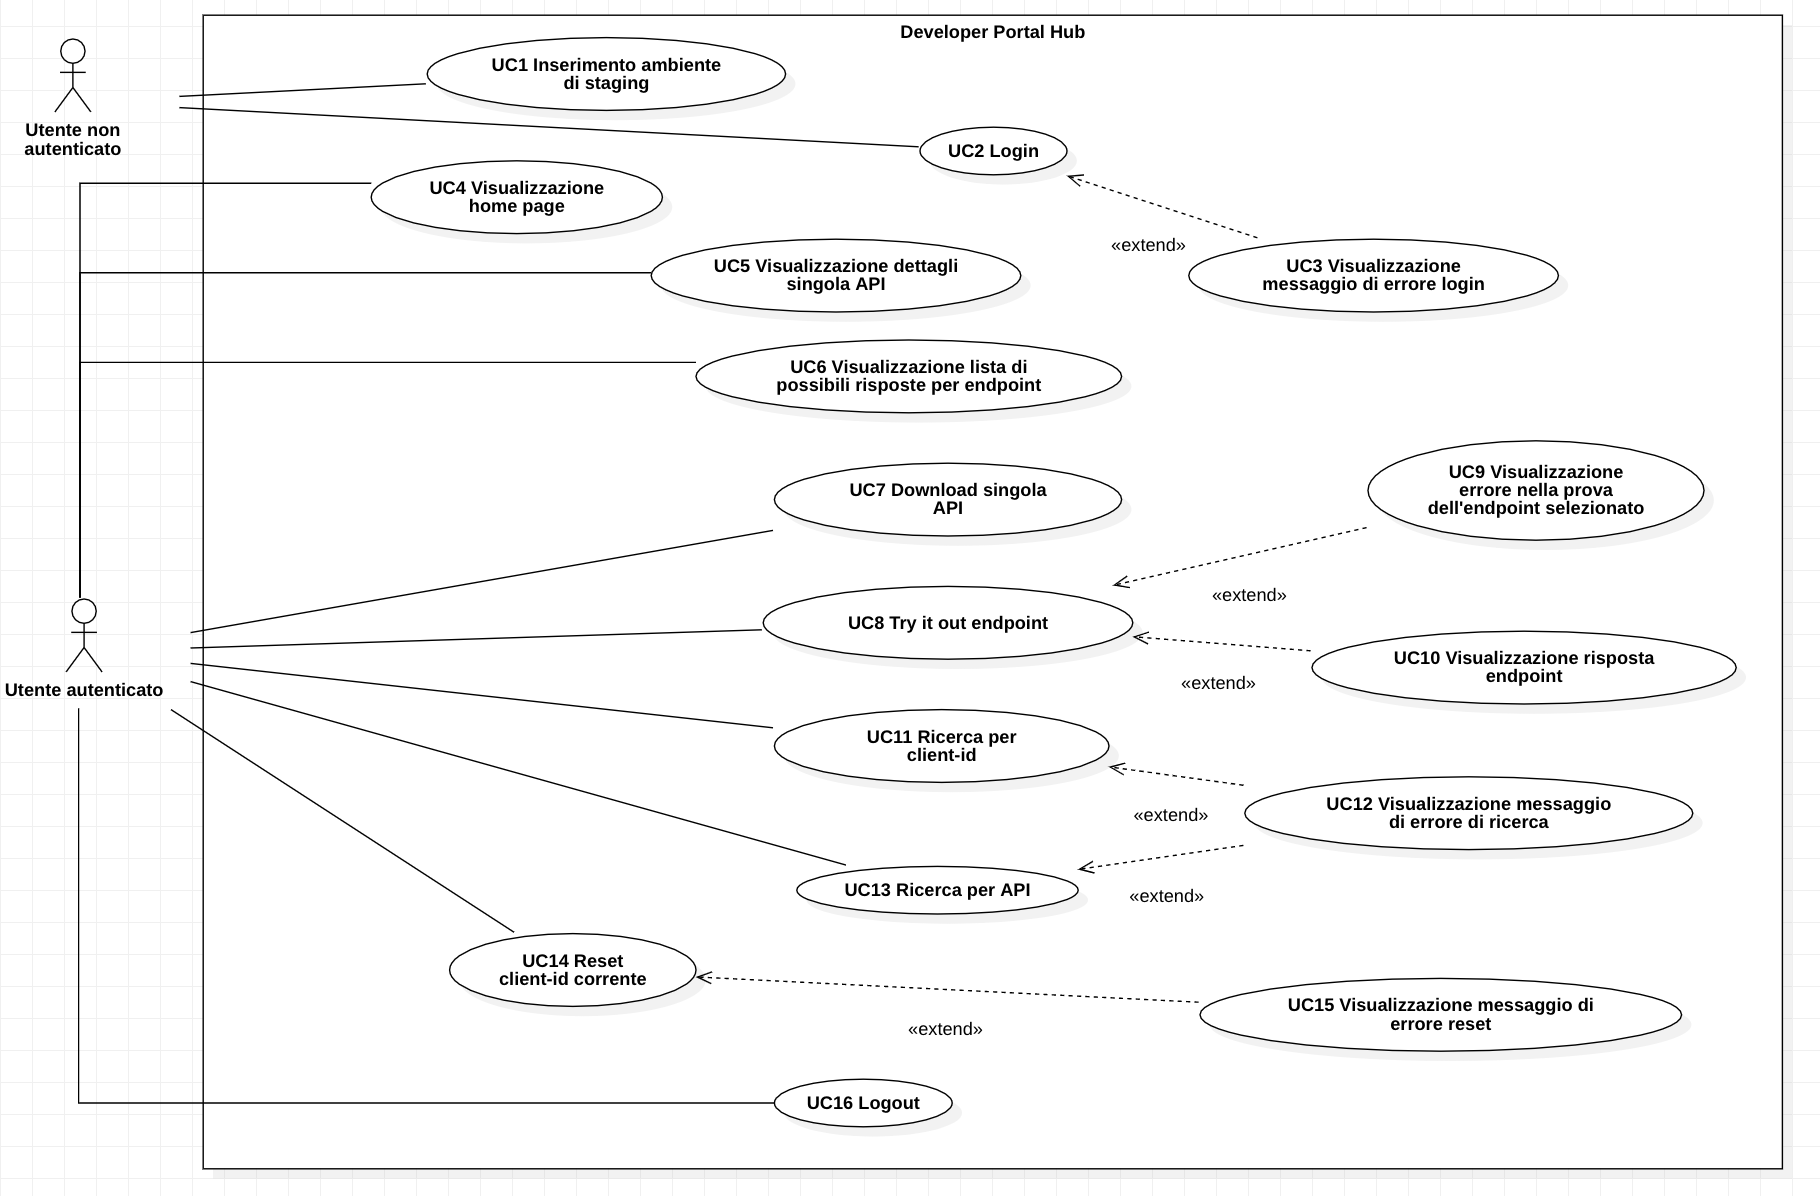
\includegraphics[width=0.9\columnwidth, alt={Scenario principale dei casi d'uso individuati}]{images/usecase/riassunto.jpg}
    \caption{Scenario principale}\label{fig:usecase-scenario-principale}
\end{figure}\\

% \clearpage


% UC 1 - Inserimento ambiente di staging
\begin{usecase}{1}{Inserimento ambiente di staging}\label{uc:inserimento-ambiente-di-staging}
    \usecaseactors{Utente non autenticato}
    \usecasepre{L'utente non è autenticato e non ha ancora avviato l'applicazione web}
    \usecasedesc{L'utente vuole avviare l'applicazione web e deve scegliere in che ambiente di staging farlo}
    \usecasepost{L'utente avvia l'applicazione nell'ambiente di staging scelto}

    \usecasemain{}
        \begin{enumerate}
            \item L'utente seleziona il link del portale a seconda dell'ambiente di staging che vuole avviare (development, quality e production)
        \end{enumerate}

\end{usecase}

% UC 2 - Login
\begin{usecase}{2}{Login}\label{uc:login}
    \usecaseactors{Utente non autenticato}
    \usecasepre{ L'utente possiede un account valido per autenticazione tramite microsoft 365 che appartiene al gruppo autorizzato per il login al sistema. Inoltre l'utente non è autenticato e si trova nella pagina di login}
    \usecasedesc{L'utente vuole accedere al sistema e deve inserire le proprie credenziali per accedervi}
    \usecasepost{L'utente è autenticato correttamente e può procedere con l'utilizzo di tutte le funzionalità disponibili all'interno del sistema}

    \usecasemain{}
        \begin{enumerate}
            \item L'utente inserisce la propria e-mail;
            \item L'utente inserisce la propria password.
        \end{enumerate}

    \usecaseext{}
    \begin{enumerate}
        \item Visualizzazione messaggio di errore login UC3.
    \end{enumerate}

    \usecasegen{}
    \begin{enumerate}
        \item Inserimento e-mail UC2.1;
        \item Inserimento password UC2.2.
    \end{enumerate}

\end{usecase}

\begin{figure}[!ht] 
    \centering 
    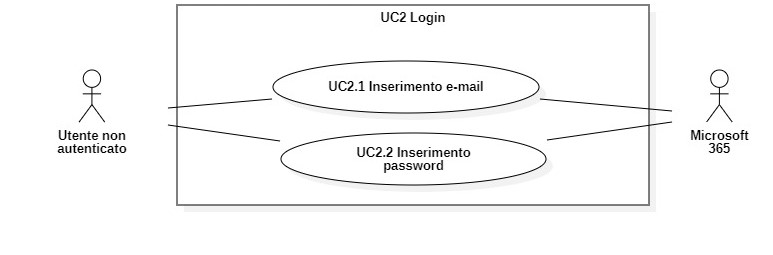
\includegraphics[width=0.9\columnwidth, alt={Caso d'uso relativo al login}]{images/usecase/UC2.jpg}
    \caption{UC2 Login}\label{fig:uc:login}
  \end{figure}
  
%   \newpage


% UC 2.1 - Inserimento e-mail
\begin{usecase}{2.1}{Inserimento e-mail}\label{uc:inserimento-email}
    \usecaseactors{Utente non autenticato}
    \usecasepre{L'utente possiede un account valido per autenticazione tramite microsoft 365 che appartiene al gruppo autorizzato per il login al sistema. Inoltre l'utente non è autenticato e si trova nella pagina di login}
    \usecasedesc{L'utente deve inserire la propria e-mail per autenticarsi al sistema}
    \usecasepost{L'utente ha inserito la propria e-mail, può quindi procedere a completare il processo di autenticazione}

    \usecasemain{}
        \begin{enumerate}
            \item L'utente inserisce nell'apposito campo la propria e-mail.
        \end{enumerate}

\end{usecase}


% UC 2.2 - Inserimento password
\begin{usecase}{2.2}{Inserimento password}\label{uc:inserimento-password}
    \usecaseactors{Utente non autenticato}
    \usecasepre{L'utente possiede un account valido per autenticazione tramite microsoft 365 che appartiene al gruppo autorizzato per il login al sistema. Inoltre l'utente non è autenticato e si trova nella pagina di login}
    \usecasedesc{L'utente deve inserire la propria password per autenticarsi al sistema}
    \usecasepost{L'utente ha inserito la propria password e può concludere il processo di autenticazione}

    \usecasemain{}
        \begin{enumerate}
            \item L'utente inserisce nell'apposito campo la propria password.
        \end{enumerate}

\end{usecase}


% UC 3 - Visualizzazione messggio di errore login
\begin{usecase}{3}{Visualizzazione messggio di errore login}\label{uc:visualizzazione-errore-login}
    \usecaseactors{Utente non autenticato}
    \usecasepre{L'utente ha inserito una tra le due credenziali email o password in modo errato}
    \usecasedesc{L'utente deve inserire delle credenziali corrette per poter effettuare il login correttamente}
    \usecasepost{L'utente ha inserito una tra le due credenziali errate}

    \usecasemain{}
        \begin{enumerate}
            \item L'utente visualizza un messaggio di errore che lo informa che una delle credenziali che ha inserito per autenticarsi al portale è sbagliata.
        \end{enumerate}

\end{usecase}


% UC 4 - Visualizzazione home page
\begin{usecase}{4}{Visualizzazione home page}\label{uc:visualizzasioen-home-page}
    \usecaseactors{Utente autenticato}
    \usecasepre{L'utente è autenticato ed è stato reindirizzato alla pagina principale del portale}
    \usecasedesc{L'utente vuole visualizzare la pagina principale del portale}
    \usecasepost{L'utente ha visualizzato la pagina principale del portale}

    \usecasemain{}
        \begin{enumerate}
            \item L'utente visualizza la pagina principale del portale.
        \end{enumerate}

    \usecasegen{}
        \begin{enumerate}
            \item Visualizzazione lista APIs disponibili UC4.1;
            \item Visualizzazione client-id di default UC4.2;
            \item Visualizzazione dettagli utente autenticato UC4.3.
        \end{enumerate}

\end{usecase}

\begin{figure}[!ht] 
    \centering 
    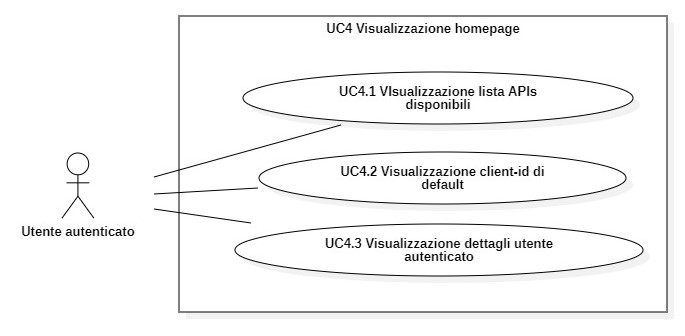
\includegraphics[width=0.9\columnwidth, alt={Caso d'uso relativo alla visualizzazione della homepage}]{images/usecase/UC4.jpg}
    \caption{UC4 Visualizzazione home page}\label{fig:uc:visualizzazione-home-page}
  \end{figure}


% UC 4.1 - Visualizzazione lista APIs disponibili
\begin{usecase}{4.1}{Visualizzazione lista APIs disponibili}\label{uc:visualizzazione-lista-apis-disponibili}
    \usecaseactors{Utente autenticato}
    \usecasepre{L'utente è autenticato ed è stato reindirizzato alla pagina principale del portale}
    \usecasedesc{L'utente vuole visualizzare la lista di API disponibili per la consultazione all'interno del portale}
    \usecasepost{L'utente ha visualizzato la lista di API disponibili all'interno del sistema}

    \usecasemain{}
        \begin{enumerate}
            \item L'utente visualizza la lista di API disponibili all'interno del sistema.
        \end{enumerate}

\end{usecase}

% UC 4.2 - Visualizzazione client-id di default
\begin{usecase}{4.2}{Visualizzazione client-id di default}\label{uc:visualizzazione-client-id-di-default}
    \usecaseactors{Utente autenticato}
    \usecasepre{L'utente è autenticato ed è stato reindirizzato alla pagina principale del portale}
    \usecasedesc{L'utente vuole visualizzare il client id di default impostato nell'ambiente corrente}
    \usecasepost{L'utente ha visualizzato il client id di default impostato nell'ambiente corrente in cui si trova}

    \usecasemain{}
        \begin{enumerate}
            \item L'utente visualizza il client id di default impostato nell'ambiente corrente in cui si trova.
        \end{enumerate}

\end{usecase}


% % UC 4.3 Visualizzazione dettagli utente autenticato
\begin{usecase}{4.3}{Visualizzazione dettagli utente autenticato}\label{uc:visualizzazione-dettagli-utente-autenticato}
    \usecaseactors{Utente autenticato}
    \usecasepre{L'utente è autenticato ed è stato reindirizzato alla pagina principale del portale}
    \usecasedesc{L'utente vuole visualizzare i propri dati personali, ovvero del proprio utente autenticato}
    \usecasepost{L'utente visualizza i dati personali del proprio account autenticato nel sistema}

    \usecasemain{}
        \begin{enumerate}
            \item L'utente visualizza le informazioni personali del proprio account autenticato nel sistema.
        \end{enumerate}

\end{usecase}

% UC 5 Visualizzazione dettagli singola API
\begin{usecase}{5}{Visualizzazione dettagli singola API}\label{uc:visualizzazione-dettagli-singola-api}
    \usecaseactors{Utente autenticato}
    \usecasepre{L'utente è autenticato e si trova nella pagina principale del portale}
    \usecasedesc{L'utente vuole visualizzare la pagina di dettaglio di una singola API}
    \usecasepost{L'utente ha visualizzato la pagina di dettaglio di una singola API tra quelle presenti nel sistema}

    \usecasemain{}
        \begin{enumerate}
            \item L'utente clicca su una delle API presenti nella lista di API disponibili all'interno del sistema.
            \item L'utente visualizza la pagina di dettaglio della singola API selezionata.
        \end{enumerate}

    \usecasegen{}
        \begin{enumerate}
            \item Visualizzazione lista endpoint disponibili UC5.1.
        \end{enumerate}

\end{usecase}

\begin{figure}[!ht] 
    \centering 
    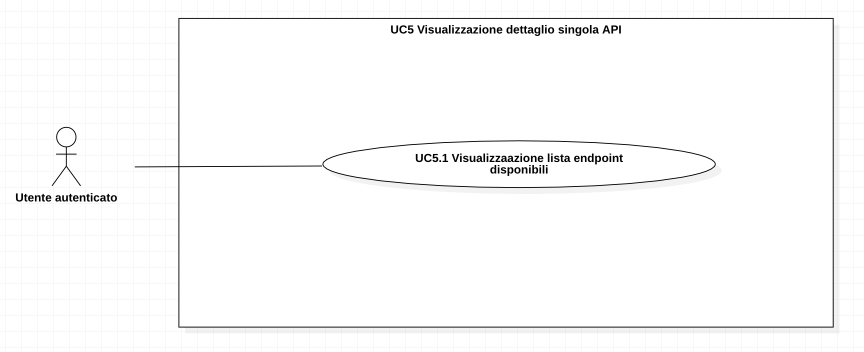
\includegraphics[width=0.9\columnwidth, alt={Caso d'uso relativo alla visualizzazione del dettaglio di una singola API}]{images/usecase/UC5.jpg}
    \caption{UC5 Visualizzazione dettaglio singola API}\label{fig:uc:visualizzazione-dettaglio-singola-api}
  \end{figure}


% UC 5.1 Visualizzazione lista endpoint disponibili
\begin{usecase}{5.1}{Visualizzazione lista endpoint disponibili}\label{uc:visualizzazione-lista-endpoint-disponibili}
    \usecaseactors{Utente autenticato}
    \usecasepre{L'utente è autenticato e sta visualizzando la pagina di dettaglio di una singola API}
    \usecasedesc{L'utente vuole visualizzare la lista completa di endpoint disponibili per l'API}
    \usecasepost{L'utente visualizza la lista completa di endpoint disponibili per l'API}

    \usecasemain{}
        \begin{enumerate}
            \item L'utente visualizza la lista completa di endpoint disponibili per l'API che ha selezionato.
        \end{enumerate}

    \usecasegen{}
        \begin{enumerate}
            \item Visualizzazione dettaglio singolo endpoint UC5.1.1.
        \end{enumerate}

\end{usecase}

\begin{figure}[!ht] 
    \centering 
    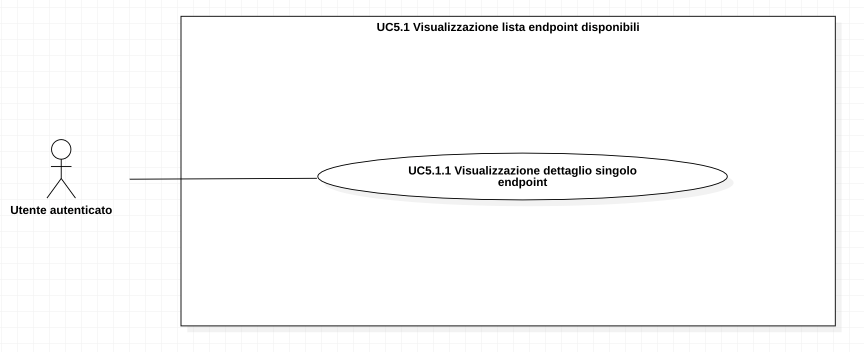
\includegraphics[width=0.9\columnwidth, alt={Caso d'uso relativo al visualizzazione della lista di endpoint disponibili}]{images/usecase/UC5.1.jpg}
    \caption{UC5.1 Visualizzazione lista endpoint disponibili}\label{fig:uc:visualizzazione-lista-endpoint-disponibili}
  \end{figure}


% UC 5.1.1 Visualizzazione dettaglio singolo endpoint
\begin{usecase}{5.1.1}{Visualizzazione dettaglio singolo endpoint}\label{uc:visualizzazione-dettaglio-singolo-endpoint}
    \usecaseactors{Utente autenticato}
    \usecasepre{L'utente è autenticato, sta visualizzando la pagina di dettaglio di una singola API contenente la lista di endpoint disponibili}
    \usecasedesc{L'utente vuole visualizzare la pagina di dettaglio di un singolo endpoint}
    \usecasepost{L'utente visualizza la pagina di dettaglio di un singolo endpoint}

    \usecasemain{}
        \begin{enumerate}
            \item L'utente clicca sullo specifico endpoint che vuole visualizzare;
            \item L'utente visualizza i dettagli disponibili per l'endpoint selezionato.
        \end{enumerate}

    \usecaseext{}
        \begin{enumerate}
            \item Visualizzazione lista di possibili risposte per endpoint UC6.
        \end{enumerate}

\end{usecase}


% UC 6 Visualizzazione lista di possibili risposte endpoint
\begin{usecase}{6}{Visualizzazione lista di possibili risposte endpoint}\label{uc:visualizzazione-risposte-endpoint}
    \usecaseactors{Utente autenticato}
    \usecasepre{L'utente è autenticato, sta visualizzando la sezione di dettaglio di un singolo endpoint}
    \usecasedesc{L'utente vuole visualizzare la lista dei possibili risultati possibili per l'endpoint selezionato}
    \usecasepost{L'utente visualizza la lista delle possibili risposte disponibili per l'endpoint che ha selezionato}

    \usecasemain{}
        \begin{enumerate}
            \item L'utente visualizza i dettagli riguardanti le possibili risposte che l'endpoint selezionato può ritornare.
        \end{enumerate}

\end{usecase}


% UC 7 Download singola API
\begin{usecase}{7}{Download singola API}\label{uc:download-singola-api}
    \usecaseactors{Utente autenticato}
    \usecasepre{L'utente è autenticato ed ha selezionato una API dalla lista di API disponibili nel sistema}
    \usecasedesc{L'utente vuole poter scaricare in formato yaml un API dal portale}
    \usecasepost{L'utente ha scaricato in formato yaml un API dal portale}

    \usecasemain{}
        \begin{enumerate}
            \item L'utente scarica il formato yaml di un API dal portale, tra quelle disponibili;
            \item Una nuova pagina si apre e il download dell'API viene eseguito;
            \item Il nome del file è già impostato con il nome dell'API scaricata.
        \end{enumerate}

\end{usecase}


% UC 8 Try it out endpoint
\begin{usecase}{8}{Try it out endpoint}\label{uc:try-it-out-endpoint}
    \usecaseactors{Utente autenticato}
    \usecasepre{L'utente è autenticato, sta visualizzando i dettagli di un singolo endpoint di un API disponibile nel portale}
    \usecasedesc{L'utente vuole poter provare l'endpoint selezionato}
    \usecasepost{L'utente ha provato l'endpoint selezionato}

    \usecasemain{}
        \begin{enumerate}
            \item L'utente ha selezionato una determinata API;
            \item L'utente ha selezionato un determinato endpoint di quell'API;
            \item L'utente ha cliccato sul pulsante per provare l'endpoint selezionato.
        \end{enumerate}

    \usecaseext{}
        \begin{enumerate}
            \item Visualizzazione errore nella prova dell'endpoint selezionato UC9;
            \item Visualizzazione risposta endpoint UC10.
        \end{enumerate}

    \usecasegen{}
        \begin{enumerate}
            \item Inserimento parametri per try it out endpoint UC8.1;
            \item Definire campi aggiuntivi per try it out endpoint UC8.2.
        \end{enumerate}

\end{usecase}

\begin{figure}[!ht] 
    \centering 
    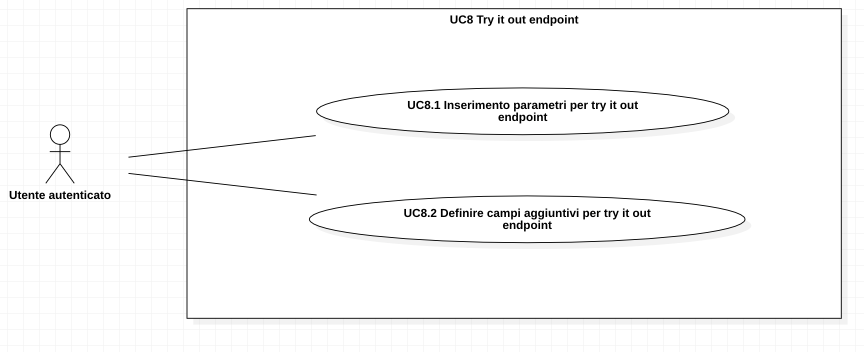
\includegraphics[width=0.9\columnwidth, alt={Caso d'uso relativo alla prova di un endpoint}]{images/usecase/UC8.jpg}
    \caption{UC8 Try it out endpoint}\label{fig:uc:try-it-out-endpoint}
\end{figure}

\newpage


% UC 8.1 Inserimento parametri necessari per la prova dell'endpoint     
\begin{usecase}{8.1}{Inserimento parametri per try it out endpoint}\label{uc:inserimento-parametri-try-it-out-endpoint}
    \usecaseactors{Utente autenticato}
    \usecasepre{L'utente è autenticato, sta visualizzando la schermata di try it out nella sezione di inserimento dei parametri}
    \usecasedesc{L'utente vuole poter inserire i parametri necessari per la prova dell'endpoint}
    \usecasepost{L'utente ha inserito i parametri necessari alla chiamata verso l'endpoint}

    \usecasemain{}
        \begin{enumerate}
            \item L'utente è nella sezione di prova dell'endpoint che ha selezionato;
            \item L'utente inserisce i parametri richiesti per la chiamata verso l'endpoint selezionato.
        \end{enumerate}

\end{usecase}


% UC 8.2 Definire campi aggiuntivi per try it out endpoint
\begin{usecase}{8.2}{Definire campi aggiuntivi per try it out endpoint}\label{uc:definire-campi-try-it-out-endpoint}
    \usecaseactors{Utente autenticato}
    \usecasepre{L'utente è autenticato, sta visualizzando la schermata di try it out nella sezione dei parametri aggiuntivi}
    \usecasedesc{L'utente vuole poter definire dei campi aggiuntivi ai parametri già esistenti, per poi andare a provare la chiamata verso l'endpoint}
    \usecasepost{L'utente ha creato dei parametri aggiuntivi per la chiamata verso l'endpoint}

    \usecasemain{}
        \begin{enumerate}
            \item L'utente è nella sezione di aggiunta dei parametri aggiuntivi, nel try it out dell'endpoint selezionato;
            \item L'utente definisce dei parametri da aggiungere a quelli già esistenti.
        \end{enumerate}

\end{usecase}

% UC 9 Visualizzazione errore nella prova dell'endpoint selezionato
\begin{usecase}{9}{Visualizzazione errore nella prova dell'endpoint selezionato}\label{uc:visualizzazione-errore-prova-endpoint-selezionato}
    \usecaseactors{Utente autenticato}
    \usecasepre{L'utente è autenticato, è nella sezione di prova di un endpoint ed ha inserito dei parametri errati}
    \usecasedesc{L'utente deve inserire dei parametri corretti per poter provare l'endpoint senza riscontrare errori} 
    \usecasepost{L'utente ha inserito dei parametri parzialmente o in modo scorretto e non può procedere con l'esecuzione della chiamata}

    \usecasemain{}
        \begin{enumerate}
            \item L'utente visualizza un messaggio di errore che lo avvisa che i parametri inseriti non sono corretti, o risultano incompleti.
        \end{enumerate}

\end{usecase}


% UC 10 Visualizzazione risposta endpoint
\begin{usecase}{10}{Visualizzazione risposta endpoint}\label{uc:visualizzazione-risposta-endpoint}
    \usecaseactors{Utente autenticato}
    \usecasepre{L'utente è autenticato, è nella sezione di prova di un endpoint ed ha inserito dei parametri corretti}
    \usecasedesc{L'utente vule visualizzare la risposta dell'endpoint}
    \usecasepost{L'utente visualizza la risposta adeguata alla chiamata verso l'endpoint, in base ai parametri inseriti}

    \usecasemain{}
        \begin{enumerate}
            \item L'utente visualizza la risposta dell'endpoint, uno tra quelle possibili contenute nella descrizione dell'endpoint. La risposta varia in base ai parametri inseriti.
        \end{enumerate}

\end{usecase}


% UC 11 Ricerca per client-id
\begin{usecase}{11}{Ricerca per client-id}\label{uc:ricerca-client-id}
    \usecaseactors{Utente autenticato}
    \usecasepre{L'utente è autenticato e sta navigando all'interno del sistema} 
    \usecasedesc{L'utente vuole poter ricercare un client-id all'interno del sistema}
    \usecasepost{L'utente effettua una ricerca per client-id e il sistema ha restituito i risultati della ricerca}

    \usecasemain{}
        \begin{enumerate}
            \item L'utente clicca il bottone per effettuare la ricerca per client-id;
            \item L'utente inserisce nell'apposito campo il client-id che vuole cercare all'interno del sistema;
            \item Il sistema ricerca il client-id inserito e restituisce i risultati della ricerca;
            \item Il sistema aggiunge l'ultima ricerca effettuata alla cronologia delle ultime ricerche.
        \end{enumerate}

    \usecaseext{}
        \begin{enumerate}
            \item Visualizzazione messaggio di errore di ricerca UC 12.
        \end{enumerate}

\end{usecase}


% % UC 12 Visualizzazione messaggio di errore di ricerca
\begin{usecase}{12}{Visualizzazione messaggio di errore di ricerca}\label{uc:visualizzazione-errore-ricerca}
    \usecaseactors{Utente autenticato}
    \usecasepre{L'utente è autenticato e ha cercato un client-id o un API inesistente nell'applicazione}
    \usecasedesc{L'utente deve inserire un client-id o un API esistenti nell'applicazione per poter effettuare la ricerca. Inoltre il client-id deve esistere per l'ambiente selezionato}
    \usecasepost{L'utente ha inserito un client-id o un API inesistente nell'applicazione e visualizza un messaggio di errore}

    \usecasemain{}
        \begin{enumerate}
            \item L'utente visualizza un messaggio di errore che lo informa che la ricerca effettuata non ha prodotto nessun risultato, indicando che ciò è dovuto al fatto
            che il client-id o l'API cercata non è presente nell'applicazione, oppure non esiste quel client-id per l'ambiente selezionato.
        \end{enumerate}

\end{usecase}


% UC 13 Ricerca per api
\begin{usecase}{13}{Ricerca per API}\label{uc:ricerca-api}
    \usecaseactors{Utente autenticato}
    \usecasepre{L'utente è autenticato e sta navigando all'interno del sistema}
    \usecasedesc{L'utente vuole poter ricercare un API all'interno del sistema}
    \usecasepost{L'utente effettua una ricerca per API e il sistema ha restituito i risultati della ricerca}

    \usecasemain{}
        \begin{enumerate}
            \item L'utente clicca il bottone per effettuare la ricerca per API;
            \item L'utente inserisce nell'apposito campo l'API che vuole cercare all'interno del sistema;
            \item Il sistema ricerca l'API inserita e restituisce i risultati della ricerca;
            \item Il sistema aggiunge l'ultima ricerca effettuata alla cronologia delle ultime ricerche.
        \end{enumerate}

    \usecaseext{}
        \begin{enumerate}
            \item Visualizzazione messaggio di errore di ricerca UC12.
        \end{enumerate}

\end{usecase}


% UC 14 Reset client-id corrente
\begin{usecase}{14}{Reset client-id corrente}\label{uc:reset-clientid}
    \usecaseactors{Utente autenticato}
    \usecasepre{L'utente è autenticato, sta navigando all'interno del sistema e ha già selezionato un client-id che non è quello di default} 
    \usecasedesc{L'utente vuole poter resettare il client-id corrente e tornare al client-id di default per l'ambiente selezionato}
    \usecasepost{L'utente ha resettato il client-id corrente e ora visualizza il client-id di default per l'ambiente selezionato}

    \usecasemain{}
        \begin{enumerate}
            \item L'utente clicca il bottone per resettare il client-id corrente;
            \item Il sistema resetta il client-id corrente ed imposta il client-id al valore di default a seconda dell'ambiente selezionato.
        \end{enumerate}

    \usecaseext{}
        \begin{enumerate}
            \item Visualizzazione messaggio di errore reset UC15.
        \end{enumerate}

\end{usecase}


% UC 15 Visualizzazione messaggio di errore reset
\begin{usecase}{15}{Visualizzazione messaggio di errore reset}\label{uc:visualizzazione-errore-reset}
    \usecaseactors{Utente autenticato}
    \usecasepre{L'utente è autenticato e ha provato a resettare il client-id corrente che è quello di default per l'ambiente selezionato}
    \usecasedesc{L'utente deve aver selezionato un client-id diverso da quello di default, per poterlo resettare}
    \usecasepost{L'utente ha provato a resettare il client-id corrente, ma risulta essere quello di default}

    \usecasemain{}
        \begin{enumerate}
            \item L'utente visualizza un messaggio di errorer che lo informa che il client-id corrente è quello di default per l'ambiente selezionato e non può essere resettato.
        \end{enumerate}

\end{usecase}


% UC 16 Logout
\begin{usecase}{16}{Logout}\label{uc:}
    \usecaseactors{Utente autenticato}
    \usecasepre{L'utente è autenticato e vuole uscire dalla sessione corrente}
    \usecasedesc{L'utente vuole effettuare il logout dal sistema}
    \usecasepost{L'utente effettua il logout dal sistema terminando la sessione corrente, non è più autenticato e viene reindirizzato alla pagina di login}

    \usecasemain{}
        \begin{enumerate}
            \item L'utente clicca il bottone per effettuare il logout;
            \item Il sistema effettua il logout dell'utente terminando la sessione e reindirizzandolo alla pagina di login.
        \end{enumerate}

\end{usecase}



\section{Tracciamento dei requisiti}

In questa sezione vengono riportati i requisiti indiduati durante il progetto di stage.
Questo capitolo si sofferma in particolare sulla classificazione dei requisiti in tre categorie principali:
\begin{itemize}
    \item Requisiti funzionali: delineano le funzionalità che il sistema deve offrire. Essi delineano le azioni specifiche che il sistema deve eseguire, le risposte attese a determinati input e le dinamiche genreali delle operazioni;
    \item Requisiti qualitativi: definiscono gli aspetti legati alla qualità, all'usabilità e alle prestazioni del sistema;
    \item Requisiti di vincolo: delineano le restrizioni e i parametri che il sistema deve rispettare durante lo sviluppo e l'implementanzione. 
\end{itemize}

Inoltre viene fatta una classificazione dei requisiti in base alla priorità assegnata a ciascun requisito.

\subsubsection{Notazione}
Ciascun requisito è identificato da un codice univoco, che segue la seguente notazione:
\begin{center}
    \textbf{R[Priorità][Tipo][Codice]}
\end{center}
  dove:
  \begin{itemize}
  \item \textbf{Priorità} indica il livello di priorità assegnato: obbligatorio (\textbf{O}), desiderabile (\textbf{D}) e opzionale (\textbf{Z}) ;
  \item \textbf{Tipo} indica il tipo di requisito: funzionale (\textbf{F}) , qualititativo (\textbf{Q}) e di vincolo (\textbf{V});
  \item \textbf{Codice} indica il codice identificativo del requisito.
  \end{itemize}

Nelle tabelle \ref{tab:requisiti-funzionali}, \ref{tab:requisiti-qualitativi} e \ref{tab:requisiti-vincolo} sono riassunti i requisiti tramite una breve descrizione accompagnata dalle fonti da cui è stato individuato il requisito per
facilitarne la tracciabilità. 

% \newpage

\subsubsection{Requisiti funzionali}

% \renewcommand{\arraystretch}{1.1} % Adjust the spacing inside the cells
% % Redefine column type to center the content
% \newcolumntype{C}[1]{>{\arraybackslash}p{#1}}

\begin{center}
\captionof{table}{Tabella del tracciamento dei requisiti funzionali}\label{tab:requisiti-funzionali}
\begin{longtable}{|c|p{0.6\textwidth}|c|}
\hline
\textbf{Requisito} & \textbf{Descrizione} & \textbf{Fonte}\\
\hline
RFO-1 &L'utente deve scegliere l'ambiente di staging & UC1 \\
\hline
RFO-2 &Il sistema deve permettere l'autenticazione ad un utente con un account valido & UC2 \\
\hline
RFO-2.1 & L'utente deve inserire la propria mail & UC2.1 \\
\hline
% \textit{username}
RFO-2.2 & L'utente deve inserire la propria password & UC2.2 \\
\hline
RFO-3 &Il sistema deve avvisare l'utente tramite un messaggio di errore che le credenziali inserite nel login sono errate & UC3 \\
\hline
RFO-4 &Il sistema deve reindirizzare l'utente alla pagina principale, dopo che il login è andato a buon fine & UC4 \\
\hline
RFO-4.1 &L'utente deve poter visualizzare la lista di API disponibili nel sistema & UC4.1 \\
\hline
RFO-4.2 &L'utente deve poter visualizzare la lista di client id di default impostata nell'ambiente di staging in cui si trova & UC4.2 \\
\hline
RFO-4.3 &L'utente deve poter visualizzare i dettagli relativi al suo account & UC4.3 \\
\hline
RFO-5 &L'utente deve poter visualizzare i dettagli relativi ad una singola API  & UC5 \\
\hline
RFO-5.1 &L'utente deve poter visualizzare la lista di endpoint disponibili all'interno del sistema & UC5.1 \\
\hline
RFO-5.1.1 &L'utente deve poter visualizzare i dettagli relativi ad un singolo endpoint di una determinata API & UC5.1.1 \\
\hline
RFO-6 &L'utente deve poter visualizzare l'elenco delle possibili risposte per il determinato endpoint selezionato & UC6 \\
\hline
RFO-7 &Il sistema deve permettere il download all'utente di una singola API & UC7 \\
\hline
RFO-8 &Il sistema deve permettere il try it out di un singolo endpoint all'utente & UC8 \\
\hline
RFO-8.1 &Il sistema deve permettere l'inserimento dei parametri necessari per il try it out di un endpoint & UC8.1 \\
\hline
RFD-8.2 &Il sistema deve permettere la possibilità di definire dei campi aggiuntivi per il try it out di un endpoint & UC8.2 \\
\hline
RFO-9 &Il sistema deve avvisare l'utente tramite un messaggio di errore che i parametri inseriti non sono corretti o incompleti & UC9 \\
\hline
RFO-10 &L'utente deve poter visualizzare la risposta dell'endpoint che ha provato & UC10 \\
\hline
RFO-11 &Il sistema deve permettere all'utente di poter effettuare una ricerca per client-id & UC11 \\
\hline
RFO-12 &Il sistema deve avvisare l'utente tramite un messaggio di errore che la ricerca effettuata non ha portato a risultati presenti nel sistema & UC12 \\
\hline
RFO-13 &Il sistema deve permettere all'utente di poter effettuare una ricerca per API & UC13 \\
\hline
RFD-14 &Il sistema deve permettedere il reset del client-id corrente & UC14 \\
\hline
RFO-15 &Il sistema deve avvisare l'utente tramite un messaggio di errore che il client-id è già di default & UC15 \\
\hline
RFO-16 &Il sistema deve permettere il logout all'utente, uscendo dalla sessione  & UC16 \\
\hline
\end{longtable}
\end{center}

\subsubsection{Requisiti qualitativi}

% \renewcommand{\arraystretch}{1.1} 
% \newcolumntype{C}[1]{>{\arraybackslash}p{#1}}

\begin{center}
\captionof{table}{Tabella del tracciamento dei requisiti qualitativi}\label{tab:requisiti-qualitativi}
\begin{longtable}{|c|p{0.6\textwidth}|c|}
\hline
\textbf{Requisito} & \textbf{Descrizione} & \textbf{Fonte}\\
\hline
RQO-1 &Il progetto deve essere accompagno da documentazione tecnica e funzionale & Interno \\
\hline
RQO-2 &La parte frontend del progetto deve essere coperto da test di unità & Interno \\
\hline
RQZ-3 &L'applicazione web deve avere un'interfaccia responsive & Interno \\
\hline
RQD-5 &L'applicativo deve essere accessibile utilizzando i principali browser & Interno \\
\hline
\end{longtable}
\end{center}


\subsubsection{Requisiti di vincolo}

% \renewcommand{\arraystretch}{1.1} 
% \newcolumntype{C}[1]{>{\arraybackslash}p{#1}}

\begin{center}
\captionof{table}{Tabella del tracciamento dei requisiti di vincolo}\label{tab:requisiti-vincolo}
\begin{longtable}{|c|p{0.6\textwidth}|c|}
\hline
\textbf{Requisito} & \textbf{Descrizione} & \textbf{Fonte}\\
\hline
RVO-1 & L'applicazione deve essere sviluppata utilizzando il framework Vue.js 3, usando Typescript come linguaggio di programmazione & UC1 \\
\hline
RVO-2 & I componenti devono essere scritti utilizzando le Composition API di Vue.js 3 & UC1 \\
\hline
RVD-3 & I componenti di base devono essere implementati utilizzando la libreria THRON Components & UC2 \\
\hline
RVZ-4 & L'interfaccia dell'applicazione deve seguire il design system THRON & UC2 \\
\hline
\end{longtable}
\end{center}